% Muc 4.3  --  phu trach: xem report/PHANCONG.md
\section{Kiến trúc CNN Lite}\label{sec:cnnlite}
\begin{goiy}
  \begin{itemize}
    \item Bốn block Conv(k=7,5,3,3) + BN + ReLU + MaxPool, GAP, FC1 $68\to32$, FC2 $32\to4$ (Bảng~\ref{tab:cnnlite}).
    \item Số liệu: 23\,408 B trọng số int8 + 212 bias int32; 1\,609\,344 MAC/nhịp; trường nhìn $\approx128$~ms.
    \item Minh hoạ một nhịp qua các tầng (Hình~\ref{fig:trace}).
  \end{itemize}
\end{goiy}
\bangcho{từng lớp: vào$\to$ra, kernel, số tham số, MAC/nhịp (xem docs/cnn\_explained.md §1)}{Kiến trúc CNN Lite và chi phí tính toán mỗi lớp.}{tab:cnnlite}

\begin{figure}[htbp]
  \centering
  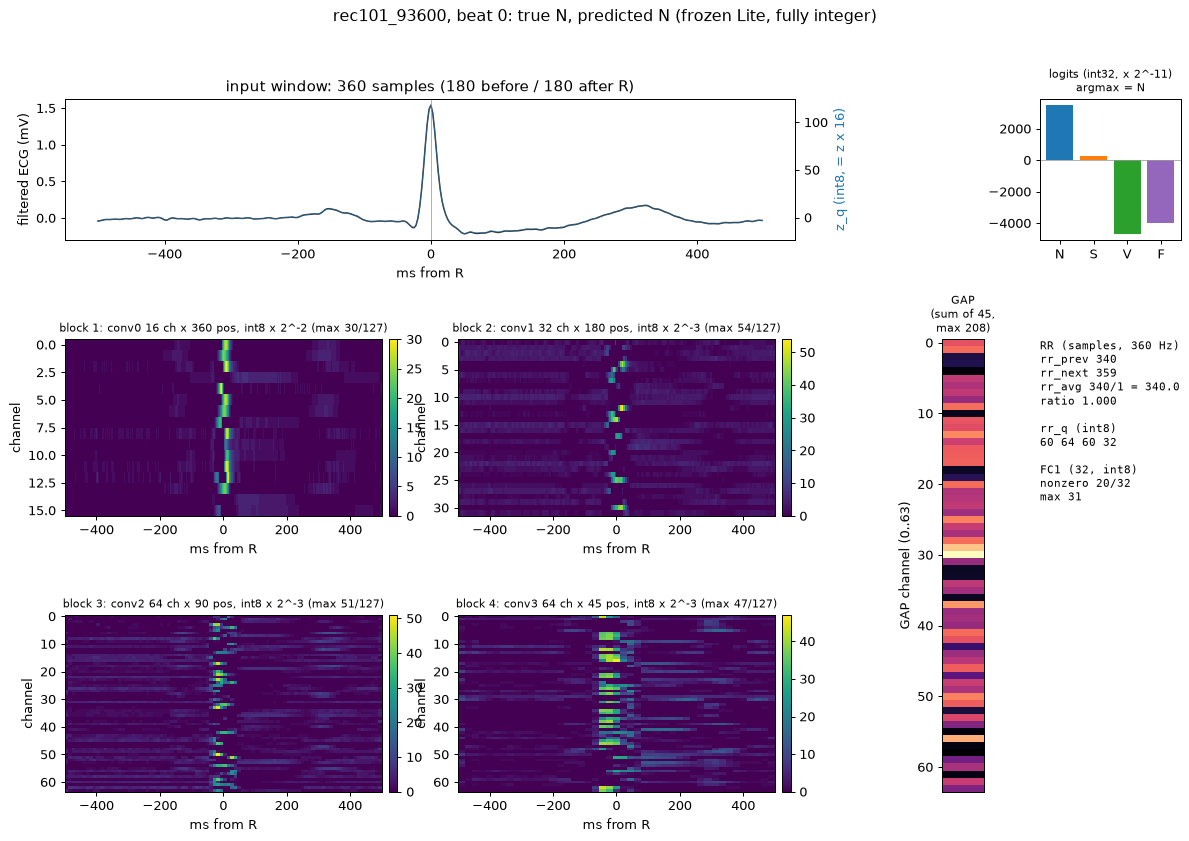
\includegraphics[width=\textwidth]{ch04_mo_hinh_cnn/trace_rec101_beat0.png}
  \caption{Một nhịp N (rec101) qua pipeline số nguyên: cửa sổ vào, feature map 4 block và logit.}\label{fig:trace}
\end{figure}
